\documentclass{spisok-article}

\title{Библиотека YC.QuickGraph: поиск путей с КС-ограничениями в графах}

\author{
    Свитков С. А., 
    студент 344 группы кафедры системного программирования СПбГУ,
    svitkovsergey@gmail.com
    
    Григорьев С. В.,
    к. ф-м н., ст. преп. кафедры системного программирования СПбГУ,
    rsdpisuy@gmail.com
}

\begin{document}

\maketitle

\begin{abstract}
	В настоящее время всё большую популярность набирает представление данных в виде графов. Более подробно стоит рассмотреть графовые базы данных, поскольку они позволяют работать с данными с помощью запросов. Но большинство языков запросов являются регулярными. Однако, регулярные языки не могут быть использованы при решении ряда задач, поскольку класс таких языков довольно сильно ограничен. Поэтому актуальной задачей является разработка средства, позволяющего использовать контекстно-свободный (далее --- КС) язык запросов к графам. Существуют теоретические работы по данной теме, однако практических реализаций мало и они обладают узкой специализацией и ограниченной функциональностью. По этой причине было решено реализовать инструмент, который позволил бы выполнять КС-запросы к ориентированным графам с помеченными ребрами, предоставлял широкий функционал и возможность представления вывода в нескольких форматах. Реализация была выполнена с использованием инструментов исследовательского проекта YaccConstructor \cite{YC}, в частности, алгоритма обобщенного синтаксического анализа GLL \cite{gll}. Результат работы --- библиотека для выполнения КС-запросов к ориентированным графам с помеченными ребрами для платформы .NET.
\end{abstract}

\section{Введение}
    Разнообразные данные могут быть представлены в виде ориентированного графа с помеченными ребрами. Такая модель имеет широкую область применения и используется в биоинформатике, при реализации графовых баз данных, в социальных исследованиях, semantic web. Работу с такими данными, как правило, выполняют с помощью языков запросов. Например, в графовой базе данных Neo4J \cite{neo4j} используется язык запросов Cypher \cite{cypher}. Он регулярный, а это означает, что класс задач, для решения которых могут быть использованы запросы на данном языке, а значит, не могут применяться, например, для решения задачи о поиске предков общего потомка при анализе генеалогического дерева, поскольку данная задача сводится к поиску строчек вида \(parent^nchild^n\), а такие строки не могут быть выведены в регулярном языке. Однако, данные строчки выводимы в языке, порожденном контекстно-свободной грамматикой с правилами \(N \to parent\,child, \,N \to parentN\, child\). Исходя из этого можно сформулировать задачу --- реализовать поддержку исполнения КС-запросов к графам. 
    
    Большая часть существующих работ по данной теме представляет лишь теорию. Те же, что реализованы на практике, предоставляют очень ограниченную функциональность, и, следовательно, применимы только в специализированных областях. Однако, реализацию хотелось бы применять для максимально широкого класса задач, решаемых с помощью КС-запросов. Исходя из этого было принято решение реализовать библиотеку для исполнения КС-запросов к графам, позволяющую представить результат запроса в различных форматах.

\section{Постановка задачи}
    Целью работы является реализация библиотеки для выполнения КС-запросов к графам в рамках платформы .NET. Полученное решение позволит представлять результат запроса в виде подграфа, множества путей, кратчайшего пути, КС-отношения (\(R = (N,\, n,\, m)\), где \(N\) --- нетерминал, из которого выводим путь из вершины \(n\) в \(m\).).
    Для достижения данной цели были поставлены следующие задачи:
    \begin{itemize}
	    \item разработать алгоритм исполнения запроса с КС-ограничениями;
        \item спроектировать расширение библиотеки YC.QuickGraph для исполнения КС-запроса;
        \item оформить результат в виде NuGet-пакета.
	\end{itemize}
\section{Существующие решения}
        \subsubsection*{Conjunctive Context-Free Path Queries}
		    В данной работе \cite{hellings} рассматривается построение обобщения существующего регулярного языка запросов к графам с помеченными ребрами CRPQ до КС-языка CCFPQ. Расширение позволяет использовать КС-грамматики вместо регулярных выражений для поиска путей в графе. Предлагаемый в статье алгоритм использует CYK для синтаксического анализа графов. Результатом исполнения запроса является КС-отношение \(R\). К минусам данной работы можно отнести отсутствие практической реализации и возможность представления результата запроса лишь в одном формате.
		\subsubsection*{Subgraph Queries by Context-free Grammars}
		    Работа \cite{subgraph} рассматривает вопрос о применении КС-запросов в различных задачах биоинформатики. Предложенный в статье подход подразумевает поиск связного подграфа, порождаемого множеством путей, строки из меток на которых выводимы из задаваемой в качестве запроса КС-грамматики. Для синтаксического анализа используется Earley parser \cite{hale2001probabilistic}. Однако из-за слишком наивного алгоритма данная реализация не может обрабатывать графы, имеющие циклы и имеет большое время исполнения запроса даже к графу небольшого размера. Кроме того, авторы предоставляют лишь один формат представления результата запроса.
        \subsection*{Ослабленный синтаксический анализ динамически формируемых выражений на основе алгоритма GLL}
	        В работе \cite{rag} предлагается алгоритм для синтаксического анализа динамически формируемого кода на основе алгоритма GLL. Предложенное решение позволяет проверять выводимость последовательсти меток на ребрах графа в задаваемой грамматике. Алгоритм, реализованный автором, позволяет обрабатывать входные данные большого размера. Так же была доказана корректность и завершаемость алгоритма. Следует отметить, что результатом работы алгоритма является лес разбора, представляемый в виде SPPF \cite{SPPF}, который можно отобразить в нужный формат вывода. Ещё одним плюсом данной работы является наличие реализации алгоритма для платформы .NET в исследовательском проекте YaccConstructor. Исходя из этого, было принято решение использовать результаты этой работы при реализации.
    
\section{Используемые инструменты}
    \subsection*{YaccConstructor}	
    Исследовательский проект YaccConstructor лаборатории языковых инструментов JetBrains, применимый для исследования и решения различных задач синтаксического и лексического анализа. Проект имеет одноименный инструмент с открытыми исходниками, который включает в себя большое количество компонентов, таких, как язык спецификаций грамматик YARD \cite{YARD}, алгоритмы для преобразования грамматик, алгоритмы для синтаксического анализа графов и др. Большая часть компонент проекта YaccConstructor реализована для платформы .NET на языке F\#. Поскольку проект имеет модульную архитектуру (рис.\ref{arch_yc}), его компоненты могут быть использованы независимо.
	    
        \begin{figure*}
            \centering
            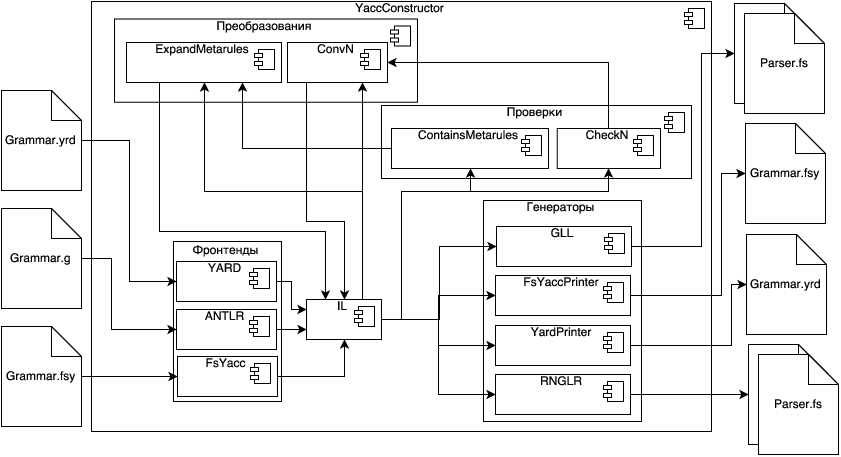
\includegraphics[width=\textwidth]{pictures/YCArch.png}
            \caption{Архитектура проекта YaccConstructor}
            \label{arch_yc}
        \end{figure*}
	    
    Более подробно рассмотрим YARD, а так же алгоритм, реализованный в работе \cite{rag}. YARD --- язык, позволяющий задавать различные типы грамматик (атрибутные, в нормальной форме Бэкуса-Наура, КС и др.). В рамках данной работы YARD используется в качестве языка запросов. 
    Обобщенный алгоритм синтаксического анализа на основе GLL позволяет осуществлять синтаксический анализ графа, результатом которого является лес разбора --- SPPF. Из полученной структуры данных с помощью различных функций можно получить результат разбора в нужном формате: в виде КС-отношения, подграфа, множества путей или кратчайшего пути.
    
    \subsection*{YC.QuickGraph}
	    Проект лаборатории языковых инструментов JetBrains YC.QuickGraph является библиотекой для работы с графами в рамках платформы .NET. YC.QuickGraph имеет средства для представления графов, различные алгоритмы для них (DFS, BFS, поиск кратчайшего пути и др.), поэтому в данной работе используется с целью предоставить пользователю возможность задавать графы.
	
\section{Реализация}
    В ходе реализации был разработан алгоритм исполнения запроса (рис. \ref{pipeline}) и архитектура (рис. \ref{arch_lib}) библиотеки, позволяющая пользователю выполнять запросы к заданным графам и получать результат в желаемом формате. Применяемый подход предоставляет пользователю возможность выполнять запросы на языке YARD к графам, реализованным в библиотеке YC.QuickGraph. Само исполнение запроса от пользователя инкапсулировано и производится средствами YaccConstructor и YC.QuickGraph (рис.\ref{pipeline}) с помощью ряда функций. Функции с высоким уровнем абстракции позволяют пользователю задать запрос просто передав в качестве параметров граф, грамматику и функцию, преобразующую объекты на ребрах графа в строки(такая функция необходима для запуска алгоритма синтаксического анализа, использумеого в решении). В свою очередь, существование функций с более низким уровнем абстракции позволяет, например, подготовить грамматику для исполнения запроса к нескольким графам. 
    \begin{figure*}
            \centering
            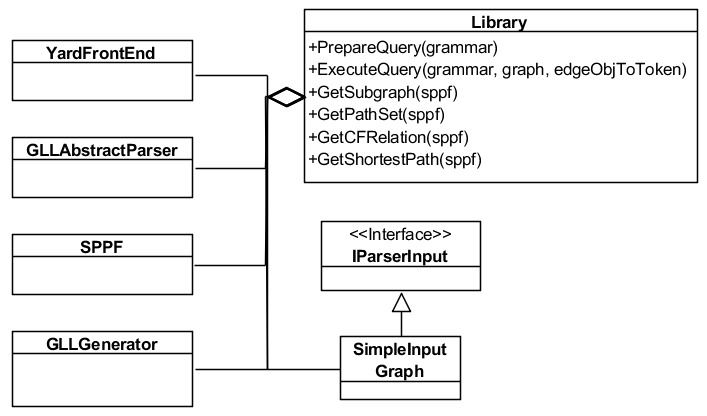
\includegraphics[width=\textwidth]{pictures/arch.png}
            \caption{Упрощенная архитектура библиотеки}
            \label{arch_lib}
    \end{figure*}
    \begin{figure*}
            \centering
            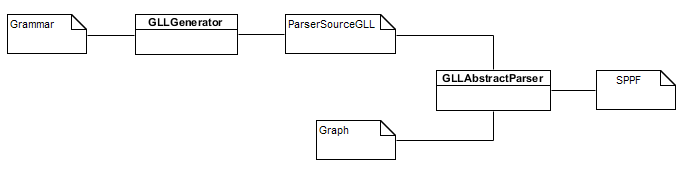
\includegraphics[width=\textwidth]{pictures/pipe.png}
            \caption{Алгоритм исполнения запроса}
            \label{pipeline}
    \end{figure*}
    Таким образом, пользователю предоставляется гибкий интерфейс с широким функционалом, что достигается за счёт возможности комбинирования различных функций. Возможность преобразования SPPF к другим форматам данных на момент написания статьи не рализована и находится в разработке. Использование .NET в качестве платформы позволяет использовать библиотеку как в программах, написанных на языке C\#, так и в программах на языке F\#. 

\section{Заключение}
    Представленное решение позволяет пользователю задавать запросы к графам с помощью контекстно-свободных грамматик, возможность использования которых существенно расширяет класс задач, решаемых с помощью такого подхода. Благодаря возможности комбинировать функции, реализованная библиотека предоствляет широкий функционал. Возможность приведения SPPF к различным форматам вывода ещё больше увеличит область применения результата работы. К предполагаемым задачам, которые могут быть решены с помощью представленной библиотеки, можно отнести различные задачи биоинформатики, социальных исследований, генеалогических исследований и др. 
    
    В ходе дальнейшей работы планируется реализовать преобразование SPPF к различным форматам, провести сравнение функциональности полученного решения с популярными средствами задания запросов к графовым структурам данных, такими, как Neo4J, Titan \cite{Titan}. Так же, для удобства пользователей, библиотеку планируется разместить в NuGet gallery. 
    
\begin{thebibliography}{8} 
\bibitem{YC} YaccConstructor, Сайт. "URL: https://github.com/YaccConstructor/YaccConstructor"
\bibitem{gsv} Григорьев, Семён Вячеславович. Cинтаксический анализ динамически формируемых программ. Diss. Ph. D. thesis/Григорьев С.
\bibitem{neo4j} Developers, Neo4J. "Neo4J." Graph NoSQL Database [online] (2012).
\bibitem{cypher} Developers, Neo4J. "Cypher" "URL: https://neo4j.com/developer/cypher-query-language/"
\bibitem{gll} Scott, Elizabeth, and Adrian Johnstone. "GLL parsing." Electronic Notes in Theoretical Computer Science 253.7 (2010): 177-189.
\bibitem{hellings} Hellings, Jelle. "Conjunctive context-free path queries." 2014.
\bibitem{subgraph} Sevon, Petteri, and Lauri Eronen. "Subgraph queries by context-free grammars." Journal of Integrative Bioinformatics (JIB) 5.2 (2008): 157-172.
\bibitem{rag} Рагозина, Анастасия Константиновна, and С. Д. Шкредов. "Ослабленный синтаксический анализ динамически формируемых программ на основе алгоритма GLL." (2016).
\bibitem{SPPF} Scott, Elizabeth. "SPPF-style parsing from Earley recognisers." Electronic Notes in Theoretical Computer Science 203.2 (2008): 53-67.
\bibitem{YARD} YARD, YaccConstructor, "URL: http://yaccconstructor.github.io/YaccConstructor/yard.html"
\bibitem{QG} YC.QuickGraph, "URL: http://yaccconstructor.github.io/QuickGraph/"
\bibitem{Titan} Chang, Chialin, et al. "Titan: a high-performance remote-sensing database." Data Engineering, 1997. Proceedings. 13th International Conference on. IEEE, 1997.

\end{thebibliography}
\end{document}
